% Standalone TikZ figure: Research Roadmap
% For Chapter 10: Conclusion and Future Directions
\documentclass[tikz,border=10pt]{standalone}
\usepackage{tikz}
\usetikzlibrary{arrows.meta, positioning, shapes.geometric, calc}

\begin{document}
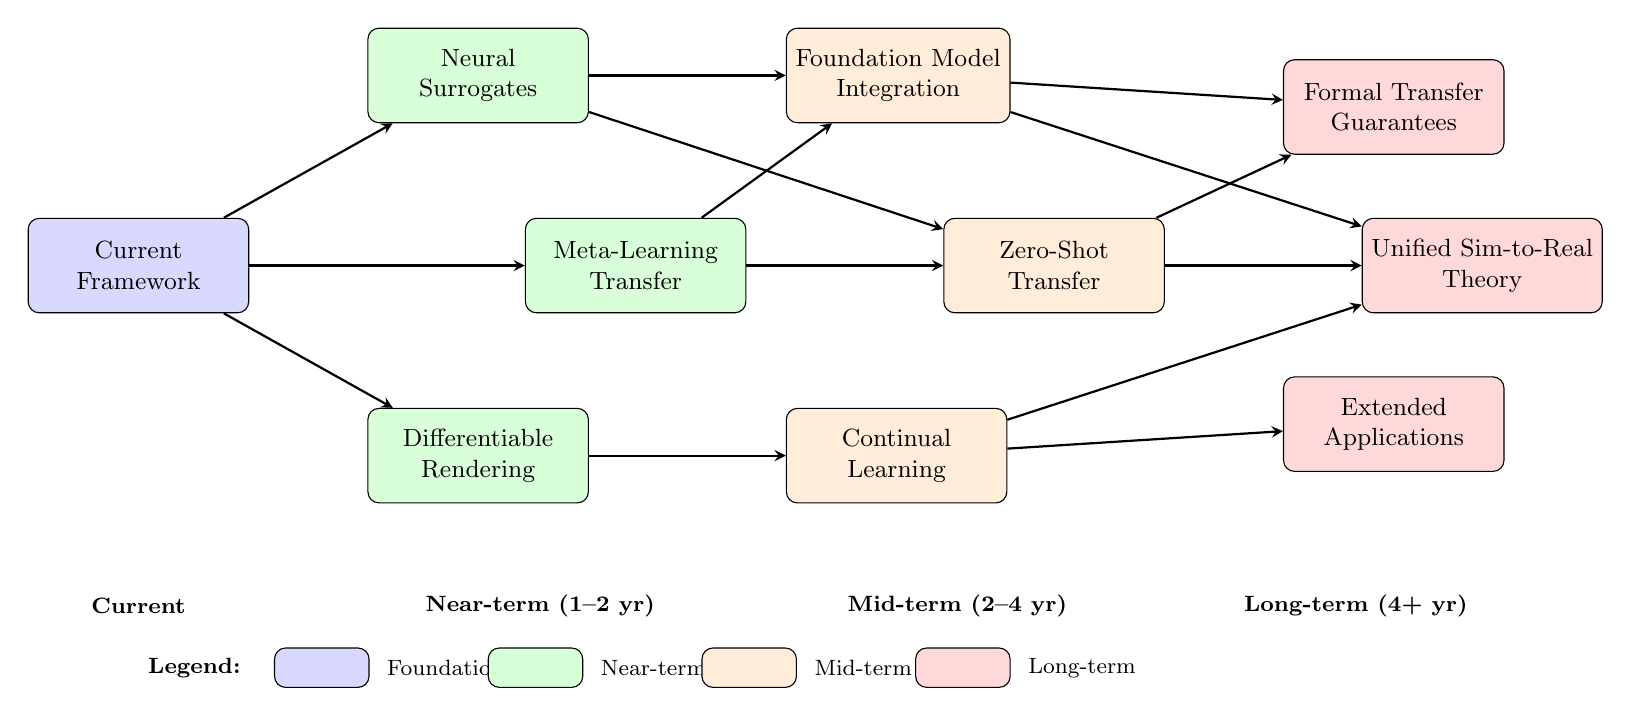
\begin{tikzpicture}[
    node distance=1.5cm and 2.5cm,
    box/.style={rectangle, draw, rounded corners, minimum width=2.8cm, minimum height=1.2cm, align=center, font=\small},
    foundation/.style={box, fill=blue!15},
    nearterm/.style={box, fill=green!15},
    midterm/.style={box, fill=orange!15},
    longterm/.style={box, fill=red!15},
    arrow/.style={->, >=stealth, thick}
]

% Foundation layer
\node[foundation] (current) {Current\\Framework};

% Near-term developments (1-2 years)
\node[nearterm, above right=1.2cm and 1.5cm of current] (surrogate) {Neural\\Surrogates};
\node[nearterm, right=3.5cm of current] (metalearning) {Meta-Learning\\Transfer};
\node[nearterm, below right=1.2cm and 1.5cm of current] (diffrender) {Differentiable\\Rendering};

% Mid-term developments (2-4 years)
\node[midterm, right=2.5cm of surrogate] (foundation) {Foundation Model\\Integration};
\node[midterm, right=2.5cm of metalearning] (zeroshot) {Zero-Shot\\Transfer};
\node[midterm, right=2.5cm of diffrender] (continual) {Continual\\Learning};

% Long-term developments (4+ years)
\node[longterm, above right=0.8cm and 1.5cm of zeroshot] (theory) {Formal Transfer\\Guarantees};
\node[longterm, right=2.5cm of zeroshot] (unified) {Unified Sim-to-Real\\Theory};
\node[longterm, below right=0.8cm and 1.5cm of zeroshot] (applications) {Extended\\Applications};

% Arrows from current to near-term
\draw[arrow] (current) -- (surrogate);
\draw[arrow] (current) -- (metalearning);
\draw[arrow] (current) -- (diffrender);

% Arrows from near-term to mid-term
\draw[arrow] (surrogate) -- (foundation);
\draw[arrow] (metalearning) -- (zeroshot);
\draw[arrow] (diffrender) -- (continual);
\draw[arrow] (surrogate) -- (zeroshot);
\draw[arrow] (metalearning) -- (foundation);

% Arrows from mid-term to long-term
\draw[arrow] (foundation) -- (theory);
\draw[arrow] (zeroshot) -- (unified);
\draw[arrow] (continual) -- (applications);
\draw[arrow] (foundation) -- (unified);
\draw[arrow] (zeroshot) -- (theory);
\draw[arrow] (continual) -- (unified);

% Timeline labels
\node[below=3.5cm of current, font=\footnotesize\bfseries] (t1) {Current};
\node[right=2.8cm of t1, font=\footnotesize\bfseries] (t2) {Near-term (1--2 yr)};
\node[right=2.2cm of t2, font=\footnotesize\bfseries] (t3) {Mid-term (2--4 yr)};
\node[right=2.0cm of t3, font=\footnotesize\bfseries] (t4) {Long-term (4+ yr)};

% Legend
\node[below=4.5cm of current, anchor=west] (legend) {\footnotesize\textbf{Legend:}};
\node[foundation, right=0.3cm of legend, minimum width=1.2cm, minimum height=0.5cm] (l1) {};
\node[right=0.1cm of l1, font=\footnotesize] {Foundation};
\node[nearterm, right=1.5cm of l1, minimum width=1.2cm, minimum height=0.5cm] (l2) {};
\node[right=0.1cm of l2, font=\footnotesize] {Near-term};
\node[midterm, right=1.5cm of l2, minimum width=1.2cm, minimum height=0.5cm] (l3) {};
\node[right=0.1cm of l3, font=\footnotesize] {Mid-term};
\node[longterm, right=1.5cm of l3, minimum width=1.2cm, minimum height=0.5cm] (l4) {};
\node[right=0.1cm of l4, font=\footnotesize] {Long-term};

\end{tikzpicture}
\end{document}
